\cfoot{Samuel Schober}
Die Nutzer können von jedem \gls{PC} mit Internetzugang auf die \gls{Webapp} zugreifen. Diese ist mit dem nutzereigenen System verknüpft. Daten bezüglich der Parameter des Aquaponik-Systems werden mit dem zentralen Server ausgetauscht und dort auf einer Datenbank persistiert. Das System wird über eine \gls{WLAN} Schnittstelle mit dem Internet verbunden und kann daher Daten senden und empfangen.\\  \\
Ein Teil der \gls{Webapp} wird auf dem lokalen System gehostet (Echtzeitdaten), während auf dem Server die Daten dauerhaft gespeichert werden um Statistiken zu ermöglichen. Die \gls{Webapp} wurde mit einem innovativem Web-Framework entwickelt. Für die Kommunikation zwischen Server und Webapp werden Websockets verwendet. Damit die \gls{Webapp} auch unterwegs benutzt werden kann und nicht nur auf dem Aquaponik-Touchscreen, wurde für die Bereitstellung dieser Applikation ein zentraler Server entwickelt, dieser Server bietet die Möglichkeit unterwegs auf die Datenauswertung des Aquaponik-Systems zuzugreifen. Diese Daten können nach Belieben als Diagramme angezeigt werden.\\  \\
Jegliche Aktoren und Sensoren des Aquaponik-Systems werden über einen Arduino \gls{SBC}  angesteuert. Dieser wiederum ist mit einem Raspberry \gls{SBC} verbunden, welcher die Daten mit einem Zeitstempel versieht, in einer Datenbank speichert und sie in späterer Folge an den zentralen Server übermittelt. Diese Verbindung funktioniert in beide Richtungen, sodass Aktoren über die Web Schnittstelle gesteuert werden können.

In Abbildung 1 sind diese Prozesse grafisch dargestellt.

\clearpage
\begin{figure}[ht]
    \centering
    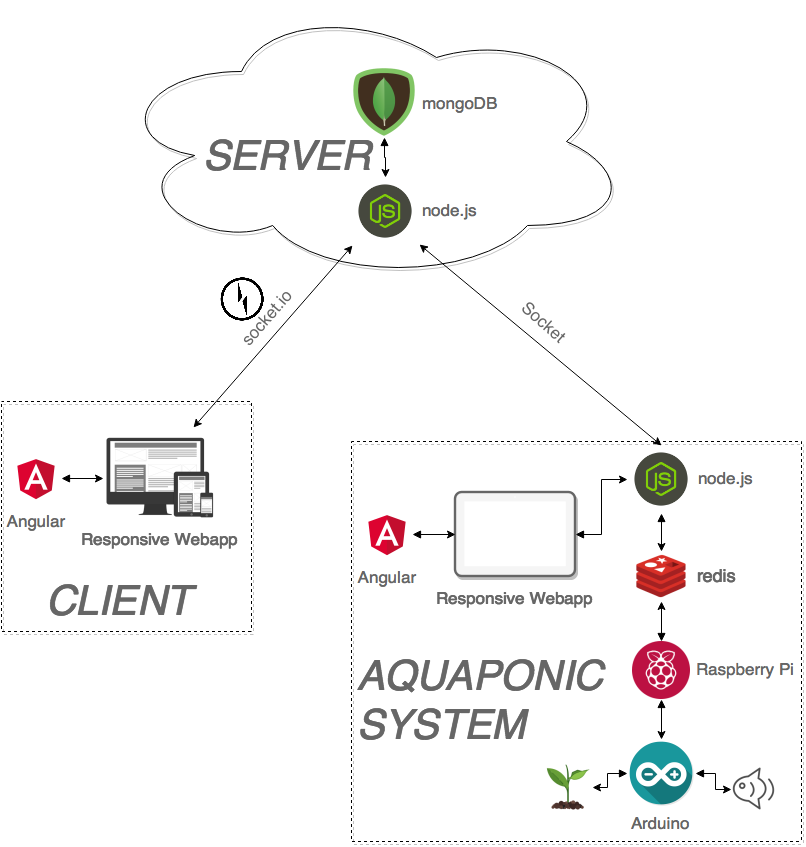
\includegraphics[height=5.5in]{images/complete_system}
	\caption{System Modell}
\end{figure}